\documentclass[11pt]{article}
\usepackage[margin=1in]{geometry}
\usepackage[T1]{fontenc}
\usepackage[utf8]{inputenc}
\usepackage{lmodern,microtype}
\usepackage{amsmath,amssymb,mathtools,bm}
\usepackage{booktabs,longtable,array,tabularx}
\usepackage{enumitem}
\usepackage{xcolor}
\usepackage{listings}
\usepackage{xurl}
\usepackage{tikz}
\usetikzlibrary{arrows.meta,positioning,shapes.geometric}
\usepackage[colorlinks=true,linkcolor=blue!55!black,urlcolor=blue!55!black]{hyperref}
\usepackage{bookmark}
\hypersetup{pdftitle={Autoformalism: Mathematical Algorithm Specification},
  pdfauthor={Autoformalism project},
  pdfsubject={Construction, fitting, feedback, and optional scientific judging}}
\def\UrlFont{\ttfamily\small}
\setlength{\emergencystretch}{3em}
\setlist{itemsep=3pt,topsep=5pt}
\newcommand{\R}{\mathbb{R}}
\newcommand{\Dtr}{\mathcal{D}_{\mathrm{tr}}}
\newcommand{\Dva}{\mathcal{D}_{\mathrm{va}}}
\newcommand{\Dte}{\mathcal{D}_{\mathrm{te}}}
\newcommand{\M}{\mathcal{M}}
\newcommand{\Loss}{\mathcal{L}}
\newcommand{\ind}{\mathbf{1}}
\newcommand{\unknown}{\bot}
\newcommand{\PASS}{\mathsf{P}}
\newcommand{\FAIL}{\mathsf{F}}
\newcommand{\UNK}{\mathsf{U}}
\newcommand{\NA}{\mathsf{N}}
\DeclareMathOperator*{\argmin}{arg\,min}
\DeclareMathOperator{\diag}{diag}
\DeclareMathOperator{\clip}{clip}
\DeclareMathOperator{\sgn}{sgn}
\lstset{basicstyle=\ttfamily\small,columns=fullflexible,keepspaces=true,
  breaklines=true,frame=single,rulecolor=\color{black!20},
  backgroundcolor=\color{black!2},showstringspaces=false}

\title{Autoformalism: Mathematical Specification of the\protect\\
Construction, Fitting, Feedback, and Scientific-Judging Pipeline}
\author{Implementation-aligned technical description}
\date{17 September 2026}

\begin{document}
\maketitle
\begin{abstract}
Autoformalism searches for a task-sufficient continuous-time model using a public
scientific specification, partially observed training trajectories, a language-model
proposer, deterministic executable-model checks, and numerical parameter fitting.
This document specifies the candidate representation, causal initial conditions,
training objective, collocation and sensitivity refinement, bounded model revision,
validation selection, and the optional paired scientific judge. It distinguishes
the current judge-free review/continuation workflow from the separately versioned
hybrid-judge selection policy. All optimization and scoring equations below are
definitions of implemented procedures or explicitly identified local numerical
approximations; none implies global optimization, identifiability, or certified
scientific recovery.
\end{abstract}
\tableofcontents
\newpage

\section{Scope and version boundaries}
\label{sec:scope}

The principal algorithm described here is staged construction followed by bounded
training-only fitting and validation-selected revision, as implemented by
\path{review_deadline_pipeline.py} and the version-3--5 continuation interfaces.
These campaigns use open rollouts, learned causal initialization, and a frozen
single-output collocation/refinement profile. Their scientific judge is off.
Sections~\ref{sec:judge}--\ref{sec:hybrid-selection} give the complete optional
paired-judge scoring and incumbent-relative selection rules. Enabling that
controller changes the experiment protocol; it is not an implicit step of the
judge-free campaigns.

Earlier repository paths also support one-step observed-state resets, general
bounded-rollout fitting, pruning, and other search policies. Those capabilities
must not be silently combined into an account of the current open-rollout
experiment. In particular, this description does not insert pruning, a
train-plus-validation final refit, or automatic numerical-budget extensions into
the current review loop. An experiment manifest fixes the actual policy.

The mathematical model notation permits multiple targets. The frozen
\path{collocation-single-target-v2} integration described in
Section~\ref{sec:fitting} supports exactly one observed target. General notation
does not assert a deployed multi-target collocation adapter.

The source inspection underlying this document used the checkout based at commit
\path{a067b835d6354b595518f906ab95bbf26fbb86c8}. An implementation/source map is
provided in Appendix~\ref{sec:sources}. Historical experiment roots retain their
own code, prompts, budgets, and interpretation.

For reproducibility, the review campaign's proposer configuration is
GPT-OSS-20B with low reasoning, temperature $0.2$, a 32,768-token serving context,
and an 8,192-token maximum output per request. Its construction budget is bounded
by 128 physical requests, 524,288 charged tokens, and three attempts per step;
later visits impose their own three-request revision cap. The optional frozen
paired-judge development configuration uses GPT-OSS-120B, low reasoning,
temperature $0.2$, and a 6,144-token output cap, with at most ten physical
provider attempts per logical stage. These are operational configurations, not
mathematical constants of Autoformalism, and an inherited experiment manifest
must be inspected before applying them to another campaign.

\section{Data, information access, and prediction semantics}
\label{sec:data}

Let $S$ be the public scientific specification. It identifies target channels,
permitted external inputs, supplied auxiliary channels, fixed covariates, and
task requirements. Let $\Dtr$, $\Dva$, and $\Dte$ denote distinct training,
validation, and held-out test splits. A trajectory $r$ consists of
\begin{equation}
 D_r=\left\{t_{ri},y_{ri},u_{ri},a_{ri}\right\}_{i=0}^{n_r-1},\quad c_r,
 \qquad t_{r,i+1}>t_{ri},
\end{equation}
where $y\in\R^q$ contains observed targets, $u$ external inputs, $a$ permitted
auxiliaries, and $c_r$ fixed public covariates. The vector $w_r(t)$ collects
exactly the time-dependent inputs/auxiliaries allowed by $S$.

For the present open-rollout protocol, prediction is
\begin{equation}
 \widehat y_r(t)=\operatorname{Predict}
 \bigl(\M,\theta;y_r(t_{r0}),w_r(\cdot),c_r\bigr).
 \label{eq:prediction-input}
\end{equation}
Later measured targets $y_r(t_{ri})$, $i>0$, are labels for fitting or scoring;
they are not forcing functions or state-reset values. A generated state or
algebraic variable named after a target is evaluated from the model, not read
from the future target column. A supplied auxiliary trajectory may be used only
under its public availability contract. Such predictions can be conditional on
auxiliary paths without constituting an autonomous simulation of every subsystem.

The current fitter uses the production forcing convention. On a permitted
linearly interpolated channel and sample interval,
\begin{equation}
 w_r(t)=(1-\alpha)w_{ri}+\alpha w_{r,i+1},\qquad
 \alpha=\frac{t-t_{ri}}{t_{r,i+1}-t_{ri}}.
 \label{eq:forcing}
\end{equation}
This equation does not authorize interpolation of target labels. Integration
respects the forcing segmentation used by the production simulator.

\paragraph{Division of information.}
The constructor receives $S$ and, in the full arm, a descriptive training packet.
Parameter estimation and residual feedback use training data only. Validation
selects retained model--parameter pairs but is not an objective inside a fitting
allocation. The paired scientific judge receives public model/specification
content, not numerical fit metrics or trajectories. Test data do not enter any
of these stages. After an explicit freeze, a separate held-out evaluation may
score the frozen artifacts without reopening discovery.

\section{Candidate models and their executable interpretation}
\label{sec:model}

\subsection{Dynamic, algebraic, and observation components}
A candidate is a typed object
\begin{equation}
 \M=(X,A,E,H,I,P,C),
\end{equation}
with dynamic-state inventory $X$, algebraic inventory $A$, directed interaction
structure $E$, observation expressions $H$, initialization rules $I$, parameter
declarations $P$, and public/runtime contracts $C$. After resolving algebraic
dependencies in topological order, its executable form, for $x_r(t)\in\R^d$, is
\begin{align}
 \dot x_r(t)&=F_{\M}\bigl(t,x_r(t),w_r(t),c_r;\theta\bigr),\\
 a^{\M}_{rj}(t)&=G_{\M,j}
   \bigl(t,x_r(t),a^{\M}_{r,<j}(t),w_r(t),c_r;\theta\bigr),\\
 \widehat y_r(t)&=H_{\M}\bigl(t,x_r(t),w_r(t),c_r;\theta\bigr).
 \label{eq:model}
\end{align}
Here $a^{\M}$ denotes generated algebraic quantities, distinct from supplied
auxiliary observations $a$. Algebraic cycles are rejected by this explicit
expression model; it is not a general implicit differential-algebraic solver.
The output map $H_{\M}$ includes algebraic substitution.

A variable's declared type determines whether its RHS defines a derivative or
an algebraic value. The proposer need not write an assignment in the RHS field.
For a dynamic variable $v$, the interpretation is $\dot v=\mathrm{RHS}$; for an
algebraic variable, it is $v=\mathrm{RHS}$. A stage-specific, unambiguous assignment
wrapper can be normalized when its target matches the selected component.
A mismatched target or contradictory dynamic/algebraic declaration requires a
diagnostic; the runtime does not guess which variable the proposer intended.

\subsection{Topology and interaction functions}
For each modeled quantity $v$, the topology declares a collection of hyperedges
\begin{equation}
 e=(v,\mathcal S_e,s_e),\qquad
 s_e\in\{+1,-1,\mathsf{unrestricted}\},
\end{equation}
where $\mathcal S_e$ is the permitted scientific source set. An interaction
``slot'' is one such hyperedge, not an entire state or a universal one-variable
function. With fixed signs, the assembled equation has the form
\begin{equation}
 \operatorname{LHS}(v)=\sum_{e:\operatorname{dest}(e)=v}
 s_e f_e(z_{\mathcal S_e};\theta_e).
 \label{eq:assembly}
\end{equation}
An outer gain, when present, is part of $f_e$; it must not be multiplied in a
second time by this notation. An unrestricted interaction preserves its supplied
signed expression instead of imposing $s_e\in\{+1,-1\}$.
For example, topology $\{x_2,x_3;+\},\{x_4;-\}$ permits
\begin{equation}
 \dot x_1=k_1f_1(x_2,x_3)-k_2f_2(x_4).
\end{equation}
Adding $x_3$ inside $f_2$ changes the interaction structure and therefore requires
an authorized structural revision rather than silent deletion of that dependency.

Under the topology-owned-sign policy, explicit redundant outer minus factors are
removed from a fixed-sign interaction before assembly. Thus, in a negative slot,
the reply $-k x^2$ becomes the function $k x^2$ and contributes $-k x^2$ once.
The normalizer follows only the outer unary/product/quotient shell. It preserves
internal differences, exponential arguments, and powers: $k(x-y)$,
$\exp(-x/\tau)$, and $(-x)^2$ retain their internal arithmetic. It does not take
an absolute value and does not prove $f_e\geq0$. The original and normalized
expressions are both recorded. Historical strict-sign policies remain distinct.

\subsection{Parameters and domain ownership}
All parameters in the current fitting adapter are global across trajectories.
Write
\begin{equation}
 \theta=(\beta,\phi)\in\Theta_{\M}
   =\{\theta:\ell_j\leq\theta_j\leq u_j,\ j=1,\ldots,p\},
\end{equation}
where $\beta$ comprises equation/output parameters and $\phi$ initializer
parameters. Infinite bounds are possible. Parameter roles and trusted constraints
determine domains; the proposer does not set numerical fitted values or optimizer
start ranges. Roles can distinguish signed coefficients, nonnegative outer gains,
positive scales/time constants, and signed or positive shape parameters. The
runtime does not force every coefficient or nonlinear shape to be positive.

Construction-local parameter names are deterministically scoped to avoid
accidental sharing across interactions. In later model-wide revisions, explicitly
shared new parameters are resolved under that revision interface. Exactly
identified inherited parameters retain their declarations and domains. Warm-start
reuse requires compatible surviving identities/declarations; it does not freeze
their numerical values against subsequent optimization.

Expressions use a restricted parsed grammar and registered mathematical
functions. Unsupported syntax, undeclared symbols, unsafe access, and invalid
domains fail the executable contract. Proposer text is never evaluated as Python.
The existing guarded-division convention replaces a denominator $d$ by
\begin{equation}
 \widetilde d=\begin{cases}
 d,&|d|\geq\epsilon_d,\\
 \epsilon_d,&0\leq d<\epsilon_d,\\
 -\epsilon_d,&-\epsilon_d<d<0,
 \end{cases}\qquad \epsilon_d=10^{-12}.
\end{equation}
This is an explicit runtime convention with a recorded warning; it is not a
scientific claim that a singular formula is valid. Other unsupported or unsafe
domains are not repaired by arbitrary clipping.

\section{Causal physical initialization}
\label{sec:initialization}

Let $o_{r0}$ be the vector of permitted initial observations, initial inputs and
auxiliaries, numeric covariates, and initial time. Physical initialization is
\begin{equation}
 x_r(t_{r0})=I_{\M}(o_{r0};\theta).
 \label{eq:initialization}
\end{equation}
A directly observed state uses its permitted initial measurement. A latent state
has an explicit boundary policy, for example
\begin{align}
 x_{rj}(t_{r0})&=\phi_j
     &&\text{(shared train-fitted value)},\\
 x_{rj}(t_{r0})&=g_j(o_{r0};\phi_j)
     &&\text{(shared train-fitted causal map)}.
\end{align}
An authorized fixed physical value is also representable. A simple map is
$g_j(o_{r0};\phi_j)=a_j+b_jy_{r0}+c_ju_{r0}$, but affine form is not mandatory.
State-local maps declare their own coefficients; they cannot silently reference
undeclared equation parameters or generated latent-state values.

Only the coefficients are shared. Two trajectories with different initial
information can have different latent initial values. Identical available
initial information gives identical deterministic initialization. Trajectory
IDs, later measured targets, and the future input schedule are not initializer
features. Independent validation/test latent initial-state fitting is forbidden.

Initialization policies are lowered to ordinary global parameters plus executable
initial expressions exactly once. A temporary zero used while assembling a draft
is not a deployable latent boundary, and a zero optimizer guess is not a fixed
physical zero. Every latent state needs a completed initialization policy before
the candidate can be fitted.

\paragraph{The search problem.}
Conceptually, structure search is a budgeted approximation to
\begin{equation}
 \min_{\M\in\mathfrak M(S)}^{\mathrm{lex}}
 \bigl(\Loss_{\mathrm{va}}(\M,\widehat\theta_{\M}),K(\M)\bigr),
 \qquad
 \widehat\theta_{\M}=
 \operatorname{BudgetedFit}(\M,\Dtr;\theta_0,B_{\mathrm{fit}}),
\end{equation}
where $\mathfrak M(S)$ is the set admitted by the active public/runtime contract.
$\widehat\theta_{\M}$ is the retained evaluated point of a finite numerical
procedure, not an assumed exact inner minimizer. Only proposed and successfully
evaluated structures are compared. No exhaustive search over $\mathfrak M(S)$,
global bilevel optimization, or posterior over structures is computed.

\section{Deterministic checking and staged construction}
\label{sec:construction}

\subsection{Executable and public contracts}
Let $V_{\mathrm{exec}}(\M,S)$ denote successful schema validation, restricted
parsing, symbol resolution, algebraic acyclicity, state-equation closure,
observation coverage, causal channel use, parameter-domain checks, and initializer
coverage. Construct a directed dependency graph with an edge $u\to v$ when the
expression defining $v$ uses modeled/public variable $u$. Observation expressions
add edges into target nodes. Reachability is transitive graph reachability.

A public target contract may require, for example,
\begin{equation}
 \operatorname{Mapped}(y_q)\ \land\
 \bigwedge_{u\in\mathcal R_q}\operatorname{Reach}(u,\operatorname{target}_q),
 \label{eq:target-contract}
\end{equation}
where $\mathcal R_q$ is derived from explicit public requirements, not hidden
reference equations. An identity output map is admissible when the corresponding
generated quantity has a valid definition. The identity alone does not establish
required composition or scientific adequacy.

Typed mechanism checks can additionally require a driver-to-target path, a
dynamic-state mediator, or a nonlinear term on an appropriate feedback path.
For the bound nonlinear-feedback pilot, the implementation searches for an
interaction with a source participating in a dependency cycle, on a relevant
public-driver/target path, and a recognized nonlinear dependence on that cycle
source after limited deterministic simplification. Formally, its necessary
structural pattern can be written
\begin{equation}
 \exists e=(v,\mathcal S_e,s_e),\ z\in\mathcal S_e:
 d\leadsto v\leadsto y_q,\quad
 v\leadsto z\to v,\quad N_{\mathrm{AST}}(f_e,z)=1.
\end{equation}
$N_{\mathrm{AST}}$ is the implemented restricted-expression test, not a general
theorem about all functions or observed dynamics. A missing eligible cycle routes
to topology revision; an eligible cycle lacking the required function form can
route to local function repair. Neither a graph path nor nonlinear syntax proves
meaningful fitted activity, stability, or recovery of the mechanism.

Each predicate has an explicit outcome, including unresolved when the public
specification does not support a determinate check. In the review controller,
an explicit failed target/mechanism predicate blocks eligibility; an unresolved
predicate is not silently converted into a scientific certificate. The
prediction-only ablation withholds scientific requirements and does not secretly
reintroduce them as selection gates.

\subsection{Construction and transactional repair}
Construction proceeds through variable inventory, equation/interaction topology,
RHS functions, and causal initializer policies. A training-only summary may
accompany every scientific stage. This packet is descriptive: sampled ranges,
initial variation, input changes, and output trends do not reveal latent states
or hidden reference equations.

Functions for the interactions of one equation can be requested together.
The runtime validates them separately and preserves accepted siblings. Only a
rejected slot is resubmitted during atomic repair. If $\mathcal E_{\mathrm{edit}}$
is the permitted edit set and $T$ a proposed transaction, acceptance requires
\begin{align}
 V_{\mathrm{exec}}(T(\M),S)&=1,\\
 V_{\mathrm{public}}(T(\M),S)&\ne\mathsf{failed},\\
 T(\M)|_{\mathcal E\setminus\mathcal E_{\mathrm{edit}}}
   &=\M|_{\mathcal E\setminus\mathcal E_{\mathrm{edit}}},
 \label{eq:transaction}
\end{align}
with analogous preservation of protected initializers and mappings. Equality
here is canonical structural equality after authorized normalization, not general
symbolic equivalence. Failed drafts retain diagnostics and leave the committed
parent intact.

Later continuation interfaces permit bounded complete-equation revisions,
new typed variables, output changes, initializer changes, and explicit removals.
This is broader than the earlier one-interaction repair pilot. New latent states
still require initialization. Version~5 treats the initial construction size
references as advisory during revision, while retaining finite response/edit
budgets, grammar checks, scientific contracts, and ablation restrictions.
Evidence citations can be audited as warnings without making an otherwise valid
mathematical edit fail; an unresolved citation does not become verified evidence.

For fixed LLM weights and frozen prompting/sampling configuration $\Lambda$,
each raw reply is a conditional proposal
$Z_k\sim p_\Lambda(\,\cdot\mid S,\mathcal C_k,E_k)$, where $\mathcal C_k$ is
the visible committed/draft model context and $E_k$ the permitted evidence and
prior diagnostics. A deterministic interpreter maps $Z_k$ to an accepted edit
or a diagnostic. On rejection, that diagnostic enters the next bounded request;
on acceptance, the transaction advances the draft. This specifies the LLM's
algorithmic role without treating its output distribution as a calibrated
scientific posterior or a guarantee of optimal proposals.

\section{Training objective and reported numerical metrics}
\label{sec:objective}

For target $q$, concatenate all its training samples and define
\begin{equation}
 \mu_q=\frac1{N_{\mathrm{tr},q}}\sum_{r,i}y_{riq},\qquad
 \sigma_q=\max\left\{
 \sqrt{\frac1{N_{\mathrm{tr},q}}\sum_{r,i}(y_{riq}-\mu_q)^2},10^{-8}\right\}.
\end{equation}
The variance uses the population denominator, as in \texttt{numpy.std} with its
default degrees of freedom. Scales are fitted once on training and reused.
The standardized prediction residual is
\begin{equation}
 e_{riq}(\theta)=\frac{\widehat y_{riq}(\M,\theta)-y_{riq}}{\sigma_q}.
 \label{eq:residual}
\end{equation}
For the current single-output profile, stack all training residuals into
$e_{\mathrm{tr}}(\theta)\in\R^{N_{\mathrm{tr}}}$. The numerical objective and
reported NMSE are
\begin{equation}
 J_{\mathrm{tr}}(\theta)=\frac12\|e_{\mathrm{tr}}(\theta)\|_2^2,
 \qquad
 \Loss_{\mathrm{tr}}(\M,\theta)=\frac{\|e_{\mathrm{tr}}(\theta)\|_2^2}
 {N_{\mathrm{tr}}}.
 \label{eq:objective}
\end{equation}
All sampled times, including the initial sample, enter the score. Longer sampled
trajectories therefore contribute more samples; this is not an equal-weight
average of trajectory NMSEs. The constant factor relating $J$ and NMSE changes
neither the exact minimizers nor their ordering within the same fitting task.
No scientific-judge score enters this least-squares objective.

Validation uses the same prediction semantics and scales:
\begin{equation}
 \Loss_{\mathrm{va}}(\M,\widehat\theta)
 =\frac1{N_{\mathrm{va}}}\sum_{r\in\Dva}\sum_i
 \left(\frac{\widehat y_{ri}(\M,\widehat\theta)-y_{ri}}{\sigma}\right)^2.
 \label{eq:val}
\end{equation}
All parameters, including initializer coefficients, are frozen at
$\widehat\theta$. An unavailable/failed rollout is an explicit status, not a
zero loss. Numerical penalties used internally to signal failed evaluations
must not compete as valid fitted solutions.

\section{The frozen collocation--refinement fitting algorithm}
\label{sec:fitting}

\subsection{Capability and budget contract}
The current adapter requires one public target, global parameters, the supported
causal boundary contract, and expressions supported by its symbolic/sensitivity
compiler. The symbolic adapter does not implement arbitrary state-constraint
penalties; unsupported constraints or expressions produce a capability failure.
It does not silently select another fitter.

The public fitting profile allocates 120 seconds to collocation initialization
and 180 seconds to feasibility screening/refinement, with a shared ceiling of
240 refinement residual evaluations. Setup, supervision, and reporting/replay
have separately recorded allowances; 300 seconds is not a guaranteed total
end-to-end wall time. The rollout solver is Radau with relative tolerance
$10^{-7}$ and absolute tolerance $10^{-9}$. Collocation uses one mesh interval
per observation interval in the frozen profile. The per-fit loss-decrease
termination option \texttt{ftol} is disabled; other native solver stopping
conditions and the frozen numerical-library version still apply.

\subsection{Collocation initialization}
For interval $[t_i,t_{i+1}]$ of length $h_i$, introduce stage states
$Z_{i1}$ and $Z_{i2}$ and let $X_i$ be its initial state node. Two-stage Radau IIA
uses
\begin{equation}
 c=\begin{pmatrix}1/3\\1\end{pmatrix},\quad
 A=\begin{pmatrix}5/12&-1/12\\3/4&1/4\end{pmatrix},\quad
 b=\begin{pmatrix}3/4\\1/4\end{pmatrix}.
\end{equation}
For each training trajectory, impose
\begin{subequations}\label{eq:collocation}
\begin{align}
 K_{i1}&=F_{\M}(t_i+h_i/3,Z_{i1},w(t_i+h_i/3),c_r;\theta),\\
 K_{i2}&=F_{\M}(t_{i+1},Z_{i2},w(t_{i+1}),c_r;\theta),\\
 Z_{i1}&=X_i+\frac{h_i}{12}(5K_{i1}-K_{i2}),\\
 Z_{i2}&=X_i+\frac{h_i}{4}(3K_{i1}+K_{i2}),\qquad X_{i+1}=Z_{i2},\\
 X_0&=I_{\M}(o_{r0};\theta),\qquad \ell\leq\theta\leq u.
\end{align}
\end{subequations}
The initializer minimizes
\begin{equation}
 \min_{\theta,\{Z_{ri1},Z_{ri2}\}}
 \sum_{r\in\Dtr}\sum_i
 \left[\frac{H_{\M}(t_{ri},X_{ri},w_r(t_{ri}),c_r;\theta)-y_{ri}}
 {\sigma}\right]^2
 \quad\text{subject to \eqref{eq:collocation}}.
 \label{eq:colloc-objective}
\end{equation}
The implementation uses CasADi/IPOPT with exact derivatives of the supported
expression graph; supported first-order-only composites use limited-memory
Hessian treatment. The native initializer uses tolerance $10^{-7}$, at most
150 iterations, and the remaining initializer CPU-time allowance. This
finite-mesh constrained problem is an initializer, not
identical to the adaptive-rollout objective at finite discretization error.

Node guesses first try an ordinary rollout within a bounded warm-up. If that
fails under the selected policy, directly observed channels can initialize their
corresponding nodes; latent node guesses repeat only the causal initial value.
These are optimization guesses, not revealed latent observations or overridden
physical boundaries. Initialization success, constraint residuals, intermediate
parameter checkpoints, timeout, and other termination states are recorded.
Only parameter values are transferred. All optimized state nodes are discarded
before reported rollout scoring.

\subsection{Feasibility screening and retained points}
An ordinary role-based start uses
\begin{equation}
 T_*=\max\left\{\operatorname{median}_r
       \operatorname{median}_i(t_{r,i+1}-t_{ri}),
       \frac{\operatorname{median}_r(t_{r,n_r-1}-t_{r0})}{10}\right\},
\end{equation}
with each median time statistic floored at $10^{-6}$ before forming the maximum.
Time constants start at $T_*$, rates at $1/T_*$, offsets at zero, and other
ordinary coefficients at $0.1$, projected into declared bounds and domains.
Explicit initializer guesses and compatible inherited values overlay these
defaults through the handoff; the complete actual start vector is sealed.

In the selected feasible-recovery profile, designed starts include three vectors
that multiply equation parameters, but preserve initializer coefficients, by
$0.1$, $0.01$, or $0.001$. These are implementation perturbations, not a claim
that every model necessarily becomes physically slower. Three additional seeded
vectors use $d_j=\max(|\theta_{0j}|,1)$ and
\begin{equation}
 \theta'_j=\begin{cases}
 \max(\theta_{0j},0.01d_j)\,10^{U_j},&
       \ell_j\geq0,\quad U_j\sim\operatorname{Uniform}[-2,1],\\
 \theta_{0j}+d_jV_j,&
       \ell_j<0,\quad V_j\sim\operatorname{Uniform}[-3,3],
 \end{cases}
\end{equation}
followed by bound clipping and exact deduplication. The implementation uses the
registered deterministic generator (default seed $20260912$). Additional
branch-targeted collocation portfolios belong to a different recovery policy
and are not inserted into this frozen feasible-recovery profile.

The ordered start list contains a converged collocation point when available,
retained collocation checkpoints (best feasible, least violation, latest), the
ordinary start, and deterministic designed starts. Exact duplicate parameter
vectors are removed. A collocation point is not considered rollout-feasible
until the full training initial-value problems have been integrated.

Screening evaluates state-only rollouts, subject to at most ten starts,
10-second individual caps, at most 40\% of the refinement time, and at most
one third of the shared residual-call budget. A usable converged collocation
point in the smooth route can end screening early. Feasible points are ranked
by their full training rollout cost, never by validation loss or by the
collocation objective alone.

Across all refinement oracles, retain
\begin{equation}
 \widehat\theta=\argmin_{\theta\in\mathcal V}J_{\mathrm{tr}}(\theta),\qquad
 \mathcal V=\{\text{evaluated points with finite, complete training rollouts}\}.
 \label{eq:retained-fit}
\end{equation}
If $\mathcal V$ is empty, fitting is unavailable. Otherwise, a finite retained
point can survive a timeout or derivative failure. The native optimizer's final
iterate and the retained best evaluated point need not coincide.

\subsection{Forward-sensitivity refinement}
For a smooth supported model let
$S_r(t)=\partial x_r(t)/\partial\theta\in\R^{d\times p}$. Differentiating the
initial-value problem yields
\begin{subequations}\label{eq:sensitivities}
\begin{align}
 \dot S_r(t)&=F_x(t)S_r(t)+F_\theta(t),\\
 S_r(t_{r0})&=\frac{\partial I_{\M}(o_{r0};\theta)}{\partial\theta},\\
 \frac{\partial\widehat y_r(t)}{\partial\theta}
   &=H_x(t)S_r(t)+H_\theta(t),\\
 [\mathcal J(\theta)]_{ri,:}
   &=\frac{H_x(t_{ri})S_r(t_{ri})+H_\theta(t_{ri})}{\sigma}.
\end{align}
\end{subequations}
Public forcing and measured initial observations are fixed data in these
derivatives. The algebraic definitions have already been substituted, so the
derivatives include their chain rules. Crucially, learned initialization maps
give a generally nonzero $S_r(t_{r0})$.

The implementation integrates $(x,S)$ and supplies $\mathcal J$ to bounded
nonlinear least squares. The local Gauss--Newton model is
\begin{equation}
 \min_{\delta}\ \frac12\|e(\theta)+\mathcal J(\theta)\delta\|^2,
 \qquad \ell\leq\theta+\delta\leq u,
\end{equation}
with the trust-region and acceptance logic of the frozen SciPy
\texttt{least\_squares} implementation. The displayed subproblem explains the
local approximation; it does not replace that library's bound-aware algorithm.
State-only feasibility is checked before derivative-based refinement. An
augmented state/sensitivity integration failure is not converted into a zero
Jacobian or a false convergence report.

\subsection{Supported nonsmooth laws and exact-cost polling}
For supported piecewise expressions, the automatic route can use derivative-free
polling; exact-cost polling is also a bounded recovery route after unavailable
sensitivities. It evaluates the unchanged full rollout loss, not a smoothed
replacement equation. At center $\theta_c$, scale
$D=\diag(\max\{|\theta_{0j}|,1\})$, radius $\rho$, and direction $d$, a poll point
is
\begin{equation}
 \theta'=\clip_{[\ell,u]}(\theta_c\pm\rho Dd).
\end{equation}
Directions include coordinate axes and, for dimension greater than one, a
reproducible orthogonal basis from a seeded Gaussian QR factorization. The initial
wide sweep uses radii $1,4,16$. Subsequent radii multiply by $1.5$ on sufficient
improvement and $0.5$ otherwise, capped at $16$. The improvement threshold is
$10^{-12}\max(1,|J_{\mathrm{anchor}}|)$; a radius below $10^{-5}$ stops polling
without a stationarity claim. Previously evaluated duplicate points are omitted.
Only finite feasible training evaluations can become incumbents. Polling shares
the remaining fitting budget and cannot grant an additional allocation.

\subsection{Replay and interpretation}
Fresh production rollouts from $\widehat\theta$ and the physical initializer
compute training and validation metrics. For the public result envelope,
\texttt{complete} denotes finite complete train/validation rollouts, not an
accuracy threshold or global optimum. Keep the following distinct:
\begin{equation}
 (\text{finite replay},\ \text{native stopping},\ \text{selected-point stopping},
 \ \text{budget exhaustion},\ \Loss_{\mathrm{tr}},\ \Loss_{\mathrm{va}}).
\end{equation}
Native termination is relevant to the selected point only when their parameter
vectors match under the recorded verification policy. A timeout alone neither
proves a missing initializer nor establishes structural infeasibility. Production
replay is also not automatically an independent-solver verification.

\section{Training evidence, model revision, and current selection}
\label{sec:controller}

\subsection{Residual evidence}
Replay the retained model at its retained parameters. For any reported
trajectory/window index set $W$, expose
\begin{equation}
 E_W=\frac1{|W|}\sum_{i\in W}e_i^2,\qquad
 b_W=\frac1{|W|}\sum_{i\in W}e_i,\qquad
 m_W=\max_{i\in W}|e_i|.
\end{equation}
The residual sign is prediction minus observation. Additional summaries include
observed/predicted ranges, endpoints, means, sampled reversals, and permitted
input regimes. Early/middle/late windows use the same global training scale;
they are descriptive partitions, not separate fitting objectives.

Reversal counting uses a running-extremum amplitude tolerance
$10^{-8}+0.01\,\operatorname{range}(y_r)$. The packet can contain at most 64
trajectory/target summaries and six detailed examples, each with at most twelve
aligned samples. Deterministic selection includes high-error, low-error, and
available zero-input examples; omissions are explicit. It carries model,
parameter, and training-data hashes. Replay NMSE must reproduce the stored
training score within the implemented relative/absolute tolerances
$10^{-5}$/$10^{-8}$ before this packet is used.

A late-time residual or a missed reversal motivates a structural hypothesis;
it does not identify a unique faulty term. The proposer receives the current
equations, retained parameter estimates, public requirements, permitted edit
scope, and numerical qualifications. It proposes mathematical changes rather
than numerically tuning the parameters in prose.

\subsection{Warm starts and validation retention}
For a revised candidate, surviving compatible parameter declarations inherit
their fitted starting values; new/changed declarations use runtime starts.
The same rule applies to initializer coefficients. These values seed a new
budgeted solve, not the internal state of the preceding optimizer.

Let $\mathcal A_r$ be the incumbent and the newly fitted trial at visit $r$ that
have passed the active executable/public/ablation checks and have finite complete
training and validation scores. The current judge-free selection is
\begin{equation}
 B_r=\argmin_{(\M,\theta)\in\mathcal A_r}^{\mathrm{lex}}
       \bigl(\Loss_{\mathrm{va}}(\M,\theta),K(\M)\bigr),
 \label{eq:selection}
\end{equation}
where $K$ counts the implemented outer additive terms in state equations and
process definitions. It is a representation-dependent tie-break, not a
representation-invariant complexity measure. An exact key tie preserves the
incumbent. An unavailable candidate has key $(+\infty,+\infty)$ and cannot
replace a valid incumbent. Thus retained validation loss is nonincreasing by
selection; that property alone is not evidence of optimizer convergence.

Each continuation visit allows up to three physical proposer requests and one
fitting allocation. A changed admissible proposal gets that allocation. An
empty/no-change reply, exhausted revision repair, or unavailable residual packet
instead uses the same allocation to refit the retained model when one exists.
After a changed trial consumes the allocation, there is no second fit merely
because it loses or fails. A rejected proposal cannot erase a valid incumbent.
The first construction can fail without producing an incumbent; that is recorded
as an unavailable lineage, not silently reconstructed on resume.

\subsection{Stopping and experiment controls}
The planned number of visits and resource budgets determine termination.
An improving fit can be granted further fitting only under an explicit
continuation/allocation protocol; the current implementation does not infer an
unlimited right to continue from a decreasing objective. Refit-only controls
spend the same per-visit fitting profile without proposer revisions. Brief-only,
no-latent, and prediction-only controls change only their declared information
or model restrictions. Imported checkpoints carry prior history but incur no
new provider cost merely by being imported.

\section{Optional scientific judge: rubric and atomic inference}
\label{sec:judge}

\subsection{Authority and inputs}
The paired judge compares two canonical candidates, $A$ and $B$, under the same
public requirement registry. Public requirements and candidate-owned claims have
different authority: a proposer annotation cannot create a public requirement or
earn mechanism coverage merely by being present. Requirements have identifiers,
positive weights, source provenance, and hard/soft/descriptive enforcement.
The implemented extractor recognizes the explicit task-required mechanism bullets
in the public prompt; it does not infer hidden obligations when the marker is absent.

Candidate identifiers, parent identifiers, and change summaries are replaced by
neutral comparison metadata. No fit score, trajectory, test result, hidden
equation, expected mutation label, or baseline identity enters the paired judge.
It is a scientific-structure assessment, not a second fit evaluator.

The response vocabulary for absolute predicates is
\begin{equation}
 \mathcal V_{\mathrm{abs}}=\{\PASS,\FAIL,\UNK,\NA\},
\end{equation}
meaning pass, fail, indeterminate, and not applicable. Each answer has a
criterion/subject key and an evidence citation. Public required mechanisms are
applicable; absence is not excused by returning not applicable. Missing, duplicate,
or invented requested units are response-contract errors, subject to bounded
format repair. The runtime, rather than the LLM, computes all aggregate scores.

\subsection{Absolute and comparative rubric}
\begin{longtable}{>{\raggedright\arraybackslash}p{0.22\textwidth}
  >{\raggedright\arraybackslash}p{0.54\textwidth}
  >{\raggedright\arraybackslash}p{0.15\textwidth}}
\toprule
Predicate family & Question/predicate & Owner\\
\midrule
\endhead
Per public requirement & Is an identifiable candidate structure representing the
requirement present? Does it have scientifically relevant influence on a requested
target? These are two separate absolute questions. & LLM\\
Task connectivity & Does each declared task input reach a requested target in the
certified dependency graph? & Runtime\\
Claim connectivity & Does each component carrying a proposer mechanism claim reach
a requested target? & Runtime\\
Latent connectivity & Does each latent state have an incoming modeled/public
driver, and does it influence a requested target? & Runtime\\
Source/sink roles & Do scientifically inferred contribution directions match
the runtime-certified outer signs? & Atomic LLM + runtime\\
Flux accounting & Are semantic fluxes free of duplicate physical contributions? & LLM + atomic evidence\\
Claim consistency & Are mechanism claims mutually consistent and supported by
the candidate equations? & LLM\\
Latent accumulators & Are accumulators justified by their dynamics and public
scientific role? & LLM\\
Delay claims & Do claimed delays have meaningful scientific representations? & LLM\\
Saturation claims & Are claimed saturation laws appropriate to their stated role? & LLM\\
\bottomrule
\end{longtable}

Graph predicates are evaluated directly, independently of LLM judgments. With no
applicable subjects (for example, no latent states), the corresponding runtime
predicate is not applicable. A graph path establishes a dependency, not the
scientific interpretation or fitted strength of that dependency.

Three additional questions are intrinsically comparative:
\begin{enumerate}
 \item Which candidate is more parsimonious while satisfying the public task?
 \item Which requires fewer unsupported scientific assumptions?
 \item Which is more mechanistically interpretable?
\end{enumerate}
Their answer set is $\{A,B,\mathsf{tie},\UNK\}$. A comparative preference is not
converted into an absolute defect claim. These questions are distinct from the
earlier six-category continuous-score rubric.

\subsection{Stage 1: sign-blinded atomic questions}
Flatten the outer additive shell of each process/state equation into signed
occurrences
\begin{equation}
 E_v=\sum_{o\in\mathcal O_v} a_o\psi_o,\qquad a_o\in\{-1,+1\}.
\end{equation}
The runtime retains $a_o$ and sends the unsigned expression $\psi_o$, its governed
quantity, its symbols, and unsigned component context to the first LLM stage.
It also enumerates syntactically exact same-polarity repeated additive terms.
This is deterministic AST decomposition, not a general algebraic-equivalence
solver.

For each occurrence the LLM infers an expected direction $d_o$: positive,
negative, context-dependent, or insufficient-public-information. Let
$R_d=\{o:d_o=d\}$ for $d\in\{-1,+1\}$, and let $U$ contain unresolved-direction
occurrences. Define $U_d$ as those unresolved occurrences governed by a quantity
that also has an occurrence in $R_d$. The runtime's source ($d=+1$) or sink
($d=-1$) verdict is, in the following precedence order,
\begin{equation}
 v_d=\begin{cases}
 \FAIL,&\exists o\in R_d:a_o\ne d,\\
 \UNK,&U_d\ne\varnothing,\\
 \PASS,&R_d\ne\varnothing,\\
 \UNK,&U\ne\varnothing,\\
 \NA,&\text{otherwise}.
 \end{cases}
 \label{eq:atomic-role}
\end{equation}
For each exact-repeat pair, the LLM separately assesses whether the occurrences
represent the same physical contribution, distinct contributions, or an
unresolved relationship. A same-physical-contribution verdict supplies a failure
of semantic flux nonduplication. Exact repeated syntax alone does not establish
that scientific relationship.

\subsection{Stage 2: semantic assessment with atomic findings}
The second stage receives the full neutralized candidates, public requirements,
runtime graph facts, and atomic findings. It answers the remaining absolute
questions and the three comparative questions. Source/sink verdicts are supplied
by \eqref{eq:atomic-role}, rather than freely rescored. A determinate atomic
same-contribution finding overrides a contrary broad no-duplication answer with
fail. The combined response must contain exactly the requested semantic units.

These stages separate scientific interpretation of a contribution's intended
direction from reading its actual outer sign. They do not guarantee that the
LLM's interpretation is correct.

\section{Paired orientations, missing evidence, and exact judge scoring}
\label{sec:judge-scoring}

\subsection{Identity-aligned question consensus}
Run both stages for orientation $(A,B)$ and for $(B,A)$ using the same seed.
Reverse the second response back into stable candidate identities: swap absolute
candidate fields and exchange relative labels $A\leftrightarrow B$.
For each absolute or comparative unit with aligned answers $v^{(1)},v^{(2)}$,
strict question consensus is
\begin{equation}
 \overline v=\begin{cases}
 v^{(1)},&v^{(1)}=v^{(2)},\\
 \UNK,&v^{(1)}\ne v^{(2)}.
 \end{cases}
 \label{eq:consensus}
\end{equation}
Scientific disagreement does not trigger a retry or a choice of the more favorable
answer. Runtime-owned facts must agree exactly after identity alignment; a
mismatch is an integrity error.

The selected operating policy seeks one complete paired seed and allows at most
two distinct seed attempts. A terminal response failure in either orientation
discards the incomplete pair for decision purposes and retries both orientations
at the next allowed seed. All calls remain charged and logged. A successful pair
contains four logical LLM stages. Two seed attempts allow at most eight logical
stages, with separately bounded physical format/transport attempts per stage.
Thus four stages is not necessarily four physical API requests. If no complete
pair is obtained, the decision is unavailable and the optional search controller
retains the incumbent.

An orientation diagnostic is
\begin{equation}
 G=\frac12\left|D^{AB}-\widetilde D^{BA}\right|,
\end{equation}
where both unaggregated decision values have been expressed as preferences for
the same candidate. It reports order sensitivity; it is neither a posterior
uncertainty nor an additional automatic rejection threshold in strict consensus.

\subsection{Group registry and default weights}
Absolute predicates form conjunction groups. Each public non-descriptive
requirement has a group containing its representation and meaningful-influence
questions, with its registered weight (normally $1$). The remaining groups are
\begin{center}
\begin{tabularx}{\textwidth}{lXr}
\toprule
Group & Members & Weight\\
\midrule
Task connectivity & All declared task inputs reach targets & $0.50$\\
Claim integrity & Claim support, claimed-component reachability, no conflicting claims & $0.25$\\
Balance semantics & Source roles, sink roles, no semantic flux duplication & $0.50$\\
Latent validity & Incoming pathways, target influence, accumulator justification & $0.25$\\
Dynamic claims & Delay meaningfulness and saturation appropriateness & $0.25$\\
\bottomrule
\end{tabularx}
\end{center}
Group membership is generated from public requirements and the model schema;
private reference structure cannot add scoring units.

\subsection{Conjunction, partial score, and coverage}
For candidate $c$ and group $g$, let $A_{gc}$ be the member units whose verdict is
not $\NA$, and let $K_{gc}=\{j\in A_{gc}:v_{jc}\ne\UNK\}$ be the determined
units. The group complete value and partial fraction are
\begin{align}
 C_{gc}&=\begin{cases}
 0,&\exists j\in K_{gc}:v_{jc}=\FAIL,\\
 1,&|A_{gc}|>0\ \land\ |K_{gc}|=|A_{gc}|\ \land\
       \forall j\in K_{gc}:v_{jc}=\PASS,\\
 \unknown,&\text{otherwise},
 \end{cases}\\
 P_{gc}&=\begin{cases}
 \dfrac{\sum_{j\in K_{gc}}\ind[v_{jc}=\PASS]}{|K_{gc}|},&|K_{gc}|>0,\\
 \unknown,&|K_{gc}|=0.
 \end{cases}
 \label{eq:group}
\end{align}
The separate within-group coverage is $|K_{gc}|/|A_{gc}|$ when $A_{gc}$ is
nonempty, and $1$ for an entirely inapplicable group. A missing assessment is
treated as indeterminate by the scorer, although the response interface normally
rejects missing required units earlier.

To reproduce the implementation exactly, define
\begin{equation}
 \mathcal G_c^P=\{g:P_{gc}\ne\unknown\},\qquad
 \mathcal G_c^C=\{g\in\mathcal G_c^P:C_{gc}\ne\unknown\}.
\end{equation}
Then
\begin{align}
 C_c&=\frac{\sum_{g\in\mathcal G_c^C}w_g C_{gc}}
               {\sum_{g\in\mathcal G_c^C}w_g},&
 P_c&=\frac{\sum_{g\in\mathcal G_c^P}w_g P_{gc}}
               {\sum_{g\in\mathcal G_c^P}w_g},\\
 S_c&=\frac{C_c+\varepsilon P_c}{1+\varepsilon},&
 \kappa_c&=\frac{\sum_{g\in\mathcal G_c^C}w_g}
                    {\sum_{g\in\mathcal G_c^P}w_g},\qquad\varepsilon=0.05.
 \label{eq:shaped}
\end{align}
A zero denominator makes the associated score unavailable; $\kappa_c=0$ when
its denominator is zero. $S_c$ exists only if both $C_c$ and $P_c$ exist.
Completely unknown groups have $P_{gc}=\unknown$ and are excluded from both sums.
Consequently this coverage is a particular implementation diagnostic, not the
fraction of all requested predicates scientifically established. Group outcomes
and missingness must be reported alongside $S_c$.

For example, a group with verdicts $(\PASS,\UNK)$ has partial value $1$ but
unknown completeness. A group with $(\FAIL,\UNK)$ has partial value $0$ and
completeness $0$. A high shaped score cannot be read as ``all requirements pass''.
The small partial term avoids independently rewarding every atomic predicate
in addition to its conjunction group.

\subsection{Hard requirement status}
For the set $\mathcal H$ of hard groups, define
\begin{equation}
 H_c=\begin{cases}
 \FAIL,&\exists g\in\mathcal H:C_{gc}=0,\\
 \PASS,&\mathcal H\ne\varnothing\ \land\ \forall g\in\mathcal H:C_{gc}=1,\\
 \UNK,&\text{otherwise}.
 \end{cases}
 \label{eq:hard}
\end{equation}
In particular, an empty hard-group set has unknown, not vacuous pass, status in
this implementation. A hard label in this scoring protocol records authority of
the public requirement; it does not turn an LLM semantic verdict into a
deterministic proof. Executable/public feasibility checks remain separate.

\subsection{Comparative residual and pair decision}
For the three consensus comparative answers $j=1,2,3$, let
\begin{equation}
 z_j=\begin{cases}
 +1,&\overline v_j=A,\\
 -1,&\overline v_j=B,\\
 0,&\overline v_j\in\{\mathsf{tie},\UNK\}.
 \end{cases}
 \qquad R_{AB}=\frac13\sum_{j=1}^{3}z_j.
 \label{eq:comparative}
\end{equation}
Indeterminate answers remain in the denominator. For $(A,\UNK,\UNK)$,
$R_{AB}=1/3$, not $1$. The historical determined-only denominator is a different
version and must not be used to reproduce this rule.

The decision value favoring $A$ is
\begin{equation}
 D_{AB}=\begin{cases}
 +1,&H_A=\PASS\ \land\ H_B=\FAIL,\\
 -1,&H_A=\FAIL\ \land\ H_B=\PASS,\\
 \unknown,&S_A=\unknown\ \lor\ S_B=\unknown,\\
 S_A-S_B+\lambda R_{AB},&\text{otherwise},
 \end{cases}\qquad \lambda=0.25.
 \label{eq:judge-decision}
\end{equation}
The preference is $A$ if $D_{AB}>\tau$, $B$ if $D_{AB}<-\tau$, tie if
$|D_{AB}|\leq\tau$, and indeterminate if unavailable, with $\tau=0.05$.
The first two hard-status cases return their specified preference directly.
The decision magnitude is bounded by $1+\lambda$; it is not a probability or a
globally comparable model score.

\section{Optional incumbent-relative hybrid selection}
\label{sec:hybrid-selection}

This section replaces \eqref{eq:selection} only when the separately frozen hybrid
controller is enabled. The first eligible fitted model seeds the incumbent
without a pairwise call. For incumbent $I$ and challenger $C$, define the symmetric
validation preference
\begin{equation}
 f_C=\begin{cases}
 \dfrac{\Loss_{\mathrm{va}}(I)-\Loss_{\mathrm{va}}(C)}
 {\Loss_{\mathrm{va}}(I)+\Loss_{\mathrm{va}}(C)},
 &\Loss_{\mathrm{va}}(I)+\Loss_{\mathrm{va}}(C)>\epsilon_{\mathrm{tiny}},\\
 0,&\text{otherwise}.
 \end{cases}
\end{equation}
Here $\epsilon_{\mathrm{tiny}}$ is the floating-point smallest normal positive
value; the implementation clips the quotient to $[-1,1]$.
The judge returns $D_{IC}$ favoring the incumbent. Set $d_C=-D_{IC}$ and
\begin{equation}
 s_C=\begin{cases}
 \unknown,&D_{IC}=\unknown,\\
 0,&|d_C|\leq\tau,\\
 \sgn(d_C)\min\!\left(1,
 \dfrac{|d_C|-\tau}{\max(1+\lambda-\tau,\epsilon_{\mathrm{mach}})}\right),
 &|d_C|>\tau.
 \end{cases}
\end{equation}
For a frozen science weight $\omega\in[0,1]$ (the development configuration uses
$\omega=0.5$), combine
\begin{equation}
 Q_C=(1-\omega)f_C+\omega s_C.
\end{equation}
Replace the incumbent iff $Q_C$ is available and strictly positive. Exact ties
and unavailable symmetric judge evidence preserve the incumbent. These decisions
compare one challenger with its round's fixed incumbent; values computed against
different incumbents are not globally ranked. This controller uses a one-member
beam. Its scientific weighting is not active in the judge-free review experiment.

\section{Diagnosis and evidence-priority routing}
\label{sec:routing}

Deterministic repair, scientific advice, and numerical findings are separate
objects bound to an exact candidate identity. The optional
\path{repair-evidence-priority-1} policy assigns ordered support levels
\begin{equation}
 s(f)\in\{0,1,2,3\}
 =\{\text{unresolved},\text{observed},\text{corroborated},\text{certified}\}.
\end{equation}
It first excludes stale findings for a different candidate. Confirmed executable
contract blockers receive level $3$. Finite verified selected-point training
replay has level $1$; verified local stopping at that same selected point can raise
it to $2$. State-only success with augmented sensitivity failure is observed
numerical difficulty at evaluated points, not necessarily at the retained point.
Timeout or missing verification alone remains unresolved model evidence.

A scientific absolute concern receives level $2$ only when its criterion,
subject, evidence text, request identity, and supported strict paired-consensus
protocol match, with distinct underlying requests. Valid comparative preference
has level $1$ and narrower scope. Reusing identical cached requests in a self-pair
does not supply independent corroboration. Mere confidence stated in LLM prose
does not establish these support levels.

The focus set is
\begin{equation}
 \mathcal F^*=\{f:s(f)=\max_{g\in\mathcal F}s(g)\}.
\end{equation}
Equal support across categories produces joint review rather than an arbitrary
scientific-versus-numerical priority. These are prescribed routing categories,
not calibrated probabilities. Scientific and numerical findings do not become
deterministic blockers by receiving a high routing priority. This policy is
implemented as an opt-in comparison protocol; the current fixed-budget review
campaign should not be described as having automatically learned or activated
this allocation rule.

\section{Other rubric versions and post-hoc assessment}
\label{sec:posthoc}

The later target-mapping/initialization semantic questions were development
extensions, not uniformly validated additions to the calibrated paired judge.
Target-completeness trials exposed unreliable semantic judgments. The deployed
public target dependency/composition contract is therefore deterministic, as in
\eqref{eq:target-contract}; its checks are not justified by claiming those LLM
extensions succeeded. The earlier six-category scalar scientific rubric is also
a distinct historical protocol, not another term in \eqref{eq:judge-decision}.

The saved-model public mechanism audit is a newer, separate advisory rubric.
It asks two seeds of a reviewer to assess each quoted public mechanism and each
separate modeling criterion from anonymous equations and saved fitted
coefficients. Method identity, model-selection scores, rationale, and previous
graph verdicts are withheld. If its two verdicts $v_{j1},v_{j2}$ agree, their
common value is retained; disagreement or a missing review yields unresolved.
For a supplied model with $m$ required mechanism units, the supported fraction is
\begin{equation}
 P_{\mathrm{supported}}=\frac1m\sum_{j=1}^{m}\ind[v_{j1}=v_{j2}=\mathsf{pass}],
\end{equation}
with unresolved units kept in $m$, separate modeling criteria, and separate
missing-model counts. A zero-unit rubric must not be interpreted as perfect
mechanism recovery. This is an uncalibrated equation-review protocol and does not
inherit the paired judge's validation.

The newer deterministic mechanism assessment additionally separates equation
predicates, fitted public-channel activity probes, and observed validation-response
agreement. Those are post-hoc measurements on fixed artifacts, not extra fitting
objectives or hidden scientific-selection signals. No single scientific-correctness
percentage is inferred by adding these distinct quantities.

\clearpage
\section{Complete operational pseudocode}
\label{sec:pseudocode}

In the following pseudocode, \texttt{CheckRepair} applies the bounded schema,
expression, public-requirement, and transactional checks of
Section~\ref{sec:construction}. The LLM is a versioned, cached conditional
proposal mechanism, not an optimizer with a specified analytic gradient.

\noindent\begin{minipage}{\linewidth}
\begin{lstlisting}[basicstyle=\ttfamily\fontsize{9}{10.5}\selectfont,
caption={Current judge-free construction and continuation loop.}]
Inputs: public specification S, training Dtr, validation Dva,
        frozen proposer/constructor/fitter settings, visits R
Seal data identities, runtime, configuration, seeds, and budgets
Fit all normalization scales on Dtr only
E0 <- descriptive_training_packet(Dtr) if arm permits it

M <- staged_construct(S, E0,
       variables_and_types, topology_and_signs,
       RHS_functions, output_mappings, causal_initializers)
M <- CheckRepair(M, bounded_attempts, preserve_valid_siblings=True)
if no deployable eligible M:
    record unavailable lineage; stop
B <- NONE

for r = 0,...,R-1:
    if r > 0:
        packet <- reproduce_training_evidence(B, Dtr)
        if packet is available:
            draft <- bounded_proposer_revision(S, B, packet)
            changed <- CheckRepair(draft, preserve_unedited_components=True)
        else:
            changed <- UNAVAILABLE  # no unsupported proposer call
        if changed is accepted and differs canonically:
            M <- changed
        else:
            M <- B.model  # continuation-policy fallback

    theta0 <- runtime_starts(M)
    if B exists:
        overlay compatible inherited fitted parameters from B
        include every compatible initializer coefficient

    fit <- FrozenFit(M, theta0, Dtr, this_visit_allocation)
    trial <- fresh_train_and_validation_replays(M, fit.retained_theta)
    if trial is eligible and both scores are finite and complete:
        if B is NONE or (trial.val_nmse, trial.term_count)
                         < (B.val_nmse, B.term_count):
            B <- trial
    checkpoint proposal, diagnostics, fit, trial, B, costs
    if B is NONE: stop lineage

Freeze selected artifacts and complete planned/missing denominators
Return B; any held-out evaluation is a separate post-freeze operation
\end{lstlisting}
\end{minipage}
\par\medskip

\noindent\begin{minipage}{\linewidth}
\begin{lstlisting}[caption={One frozen training-only numerical allocation.}]
FrozenFit(M, theta0, Dtr, budget):
    verify adapter capabilities and physical initialization
    solve bounded Radau collocation initializer on Dtr
    retain parameter checkpoints, not optimized state trajectories
    starts <- deduplicated ordered collocation/ordinary/designed starts
    feasible <- bounded full-training state-only screening(starts)
    if smooth supported sensitivities and feasible is nonempty:
        attempt bounded least squares with analytic residual Jacobian
        record unavailable sensitivities separately from state failure
    if prescribed polling/recovery condition and budget remains:
        poll exact training rollout costs under the same shared budget
    theta <- best finite complete training evaluation across stages
    verify theta by fresh production rollout
    return theta, native stopping, selected-point qualification,
           budget status, all stage diagnostics and costs
\end{lstlisting}
\end{minipage}
\par\medskip

\noindent\begin{minipage}{\linewidth}
\begin{lstlisting}[caption={Optional paired scientific judge.}]
PairedJudge(A, B, public_requirements, frozen_scoring):
    for seed in at_most_two_registered_seeds:
        for orientation in [(A,B), (B,A)]:
            facts <- deterministic_dependency_facts(orientation)
            occurrences <- unsigned_atomic_plan(orientation)
            atomic <- cached_LLM_stage_1(requirements, occurrences)
            roles <- compare_expected_directions_to_private_actual_signs()
            semantic <- cached_LLM_stage_2(requirements, neutral_models,
                                          facts, atomic, roles)
            result[orientation] <- merge_and_validate(semantic, roles,
                                                     repeat_findings)
        if either orientation terminally failed:
            discard incomplete pair for scoring; continue
        reverse second result to stable identities
        consensus <- keep_equal_answers_else_indeterminate(results)
        require exact agreement of deterministic facts
        compute groups, shaped scores, hard status, fixed-denominator votes
        return versioned pair decision and full evidence provenance
    return UNAVAILABLE
\end{lstlisting}
\end{minipage}
\par\medskip

\begin{figure}[p]
\centering
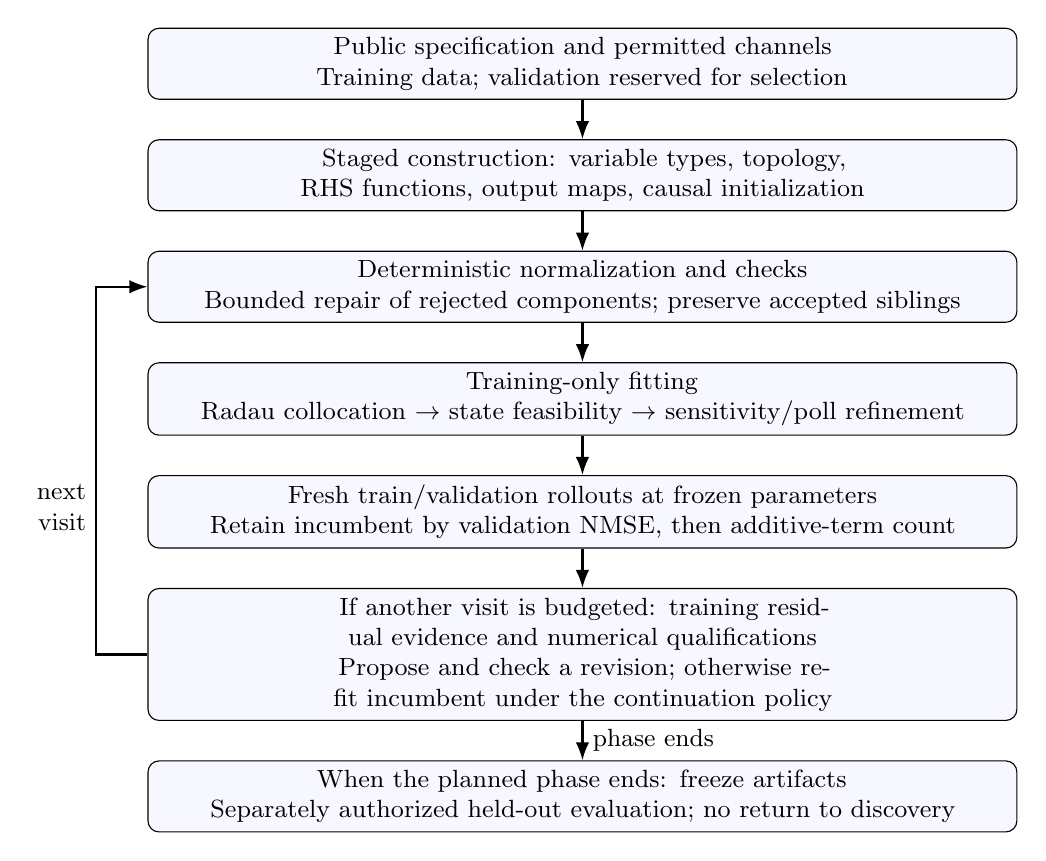
\begin{tikzpicture}[
  box/.style={draw,rounded corners,align=center,text width=10.8cm,
              minimum height=0.85cm,font=\small,fill=blue!3},
  smallbox/.style={box,text width=3.1cm,fill=orange!5},
  edge/.style={-{Latex[length=2.3mm]},thick},node distance=0.5cm]
\node[box] (data) {Public specification and permitted channels\\Training data;
  validation reserved for selection};
\node[box,below=of data] (construct) {Staged construction: variable types,
  topology, RHS functions, output maps, causal initialization};
\node[box,below=of construct] (check) {Deterministic normalization and checks\\
  Bounded repair of rejected components; preserve accepted siblings};
\node[box,below=of check] (fit) {Training-only fitting\\
  Radau collocation $\to$ state feasibility $\to$ sensitivity/poll refinement};
\node[box,below=of fit] (score) {Fresh train/validation rollouts at frozen parameters\\
  Retain incumbent by validation NMSE, then additive-term count};
\node[box,below=of score] (feedback) {If another visit is budgeted: training
  residual evidence and numerical qualifications\\Propose and check a revision;
  otherwise refit incumbent under the continuation policy};
\node[box,below=of feedback] (freeze) {When the planned phase ends: freeze artifacts\\
  Separately authorized held-out evaluation; no return to discovery};
\draw[edge] (data)--(construct);
\draw[edge] (construct)--(check);
\draw[edge] (check)--(fit);
\draw[edge] (fit)--(score);
\draw[edge] (score)--(feedback);
\draw[edge] (feedback)-- node[right,font=\small] {phase ends} (freeze);
\draw[edge] (feedback.west)--++(-0.65,0)|- node[pos=0.2,left,font=\small,
  align=right] {next\\visit} (check.west);
\end{tikzpicture}
\caption{Current open-rollout review/continuation workflow. The optional paired
judge and hybrid selection rule are specified separately; they are not silently
inserted into this judge-free experiment. A failed check or fit retains its
explicit failure status even when an incumbent survives.}
\label{fig:pipeline}
\end{figure}
\clearpage

\section{Illustrative model and identifiability boundary}
\label{sec:example}

Consider a public observed output $y$, a permitted input $u$, and a proposed
latent memory $m$:
\begin{align}
 \dot m&=k_u u-m/\tau,\\
 \dot y&=c m-d y-b\frac{y^2}{K^2+y^2},\qquad \widehat y=y,\\
 y_r(0)&=y_{r0},\qquad
 m_r(0)=\alpha+\beta y_{r0}+\gamma u_{r0}.
\end{align}
This is an illustrative model, not a benchmark reference or a preferred repair.
The parameter vector includes both equation coefficients and
$(\alpha,\beta,\gamma)$. For these three initializer coefficients,
\begin{equation}
 \frac{\partial m_r(0)}{\partial(\alpha,\beta,\gamma)}
       =(1,y_{r0},u_{r0}),\qquad
 \frac{\partial y_r(0)}{\partial(\alpha,\beta,\gamma)}=(0,0,0).
\end{equation}
These rows seed \eqref{eq:sensitivities}. The function $b y^2/(K^2+y^2)$ occupies
a negative self-feedback interaction of $y$. A redundant leading minus in that
slot is normalized before assembly. The identity observation $\widehat y=y$ is
useful because $y$ has its own generated dynamics; it is not copying later labels.
Validation uses the same learned initial map on its new $(y_{r0},u_{r0})$.

Neither a good loss nor a passing structural rubric generally identifies unique
latent coordinates. For an invertible differentiable latent change of coordinates
$z=T(x)$, corresponding dynamics and output maps satisfy
\begin{equation}
 \dot z=J_T(T^{-1}z)F(T^{-1}z,w;\theta),\qquad
 H'(z,w;\theta)=H(T^{-1}z,w;\theta),\qquad I'=T\circ I.
\end{equation}
When these transformed functions and boundaries are admissible, the models can
have identical observed predictions. Public scientific restrictions may exclude
some transformations, but the algorithm provides no general uniqueness theorem.
It seeks task-sufficient predictive and mechanistic models under its public
contracts, not recovery of a privileged hidden naming convention.

\section{Checkpoints, cost accounting, and scientific interpretation}
\label{sec:provenance}

Each stage binds its candidate, input data, configuration, source/runtime version,
and parent identity using canonical content hashes. Provider requests and replies,
raw and normalized expressions, diagnostics, fitted vectors, stage budgets,
selection decisions, and missing outcomes are retained. Completed stages resume
from their artifacts; an uncertain request delivery or interrupted numerical
attempt cannot silently receive fresh uncharged budget. A warm-start continuation
is a new explicitly allocated solve, not restoration of undocumented optimizer
internals. Cache-based resume reproduces saved decisions; stochastic fresh calls
and wall-clock-limited numerical solves are not promised bitwise-identical across
machines.

For deduplicated captured provider responses $\mathcal Q$, let
$\mathcal Q_k\subseteq\mathcal Q$ contain those with a recorded usage field
$k\in\{\mathrm{in},\mathrm{out},\mathrm{total}\}$. Observed token accounting is
\begin{equation}
 T_k^{\mathrm{observed}}=\sum_{q\in\mathcal Q_k}t_{q,k},\qquad
 U_k=|\mathcal Q\setminus\mathcal Q_k|.
\end{equation}
Report $U_k$, field coverage, and any attempts with no captured response
separately; missing usage is not zero or inferred billed usage.
Cached/reasoning token fields, when available, are subdivisions of input/output
usage, not additional tokens to add again. Repair calls count. A logical judge
stage, a transport attempt, a hosted tool call, and a numerical residual evaluation
are different cost units. Resource limits and budget charges need not equal
provider-observed token counts.

Final selection is frozen before any held-out evaluation. For the workflow
described here, the selected learned parameters and causal map remain fixed.
No claim that test evaluation has occurred follows merely from producing a
freeze artifact. Validation-adapted results are development estimates; repeated
selection on the same validation set does not create an independent test estimate.

The following implications are deliberately not made:
\begin{align*}
 \text{executable model}&\ \not\Rightarrow\ \text{scientifically correct model},\\
 \text{graph/nonlinear syntax present}&\ \not\Rightarrow\ \text{active mechanism},\\
 \text{finite replay}&\ \not\Rightarrow\ \text{good predictive accuracy},\\
 \text{native local stopping}&\ \not\Rightarrow\ \text{global optimum},\\
 \text{budget exhaustion}&\ \not\Rightarrow\ \text{structural infeasibility},\\
 \text{paired judge agreement}&\ \not\Rightarrow\ \text{independent scientific proof}.
\end{align*}

\appendix
\section{Source map and reproducibility references}
\label{sec:sources}

Paths below are relative to the project root. They identify the executable
definitions and protocol documents inspected for this explanation. Versioned
experiment manifests take precedence over generic historical documentation.

\begin{longtable}{>{\raggedright\arraybackslash}p{0.24\textwidth}
  >{\raggedright\arraybackslash}p{0.69\textwidth}}
\toprule
Topic & Source files\\
\midrule
\endhead
Current outer loop &
\path{src/autoformalism/rebuttal/review_deadline_pipeline.py};
\path{docs/REVIEW_CONTINUATION_V3.md};
\path{docs/REVIEW_CONTINUATION_V4.md};
\path{docs/REVIEW_CONTINUATION_V5.md}\\
Construction and checks &
\path{src/autoformalism/search/staged_topology_runner.py};
\path{src/autoformalism/search/staged_function_runner.py};
\path{docs/PREFIT_CONSTRUCTION_AUDIT.md};
\path{docs/PREFIT_SIGN_NORMALIZATION.md}\\
Causal initialization &
\path{src/autoformalism/search/causal_initialization.py};
\path{src/autoformalism/fitting/initialization.py};
\path{docs/CAUSAL_INITIALIZER_CONSTRUCTION.md}\\
Public requirements &
\path{src/autoformalism/targets.py};
\path{src/autoformalism/rebuttal/mechanisms.py};
\path{src/autoformalism/search/requirement_feedback.py}\\
Normalization and fitting &
\path{src/autoformalism/data/scaling.py};
\path{src/autoformalism/fitting/public_fitting.py};
\path{src/autoformalism/fitting/collocation_sensitivity.py};
\path{src/autoformalism/fitting/matching_probe.py}\\
Refinement and recovery &
\path{src/autoformalism/fitting/sensitivity_probe.py};
\path{src/autoformalism/fitting/feasibility.py};
\path{src/autoformalism/fitting/directional_poll.py};
\path{docs/FITTER_FREEZE.md}\\
Residual feedback &
\path{src/autoformalism/search/residual_evidence.py};
\path{docs/TRAINING_RESIDUAL_FEEDBACK.md}\\
Paired judge and scoring &
\path{src/autoformalism/judging/hybrid.py};
\path{src/autoformalism/judging/prompts.py};
\path{src/autoformalism/schemas/judge.py};
\path{src/autoformalism/search/hybrid_pair.py}\\
Optional hybrid controller &
\path{src/autoformalism/search/controller.py};
\path{configs/hybrid_search_objective_pilot_v2.json};
\path{docs/JUDGE_HYBRID_PROTOCOL.md}\\
Evidence-priority routing &
\path{src/autoformalism/rebuttal/repair_priority.py};
\path{docs/PREFIT_MILESTONES.md}\\
Post-hoc assessment &
\path{docs/PUBLIC_MECHANISM_AUDIT.md};
\path{docs/DETERMINISTIC_MECHANISM_ASSESSMENT.md}\\
\bottomrule
\end{longtable}

\begin{flushleft}
Representative executable checks include
\path{tests/test_review_deadline.py},
\path{tests/test_review_revision_v5.py},
\path{tests/test_causal_initialization_construction.py},
\path{tests/test_collocation_sensitivity.py},
\path{tests/test_residual_evidence.py},
\path{tests/test_hybrid_judge.py}, and
\path{tests/test_atomic_occurrence_judge.py}. The real-fit/mock-provider smoke
\path{scripts/smoke_review_continuation.py} exercises the current orchestration
without a live LLM or sealed benchmark test evaluation.
\end{flushleft}

\par\bigskip
\noindent\begin{minipage}{\linewidth}
\section{Building this document}
From the project root, create the build directory and run the
\texttt{pdflatex} command below twice with a standard TeX installation:
\begin{lstlisting}
mkdir -p /tmp/autoformalism-algorithm-tex
pdflatex -halt-on-error -interaction=nonstopmode \
  -output-directory=/tmp/autoformalism-algorithm-tex \
  docs/AUTOFORMALISM_ALGORITHM.tex
\end{lstlisting}
The second pass resolves internal references and the table of contents. The
source is self-contained; it requires no remote figures, bibliography download,
benchmark data, credentials, or shell-escape execution.
\end{minipage}

\end{document}
